



%%%%%%%%%%%%%%%%%%%%%%%%%%%%%%%%%%%%%%%%%
% Beamer Presentation
% LaTeX Template
% Version 1.0 (10/11/12)
%
% This template has been downloaded from:
% http://www.LaTeXTemplates.com
%
% License:
% CC BY-NC-SA 3.0 (http://creativecommons.org/licenses/by-nc-sa/3.0/)
%
%%%%%%%%%%%%%%%%%%%%%%%%%%%%%%%%%%%%%%%%%

%----------------------------------------------------------------------------------------
%	PACKAGES AND THEMES
%----------------------------------------------------------------------------------------

\documentclass[aspectratio=169]{beamer}

\mode<presentation> {


% The Beamer class comes with a number of default slide themes
% which change the colors and layouts of slides. Below this is a list
% of all the themes, uncomment each in turn to see what they look like.

%\usetheme{default}
%\usetheme{AnnArbor}
%\usetheme{Antibes}
%\usetheme{Bergen}
%\usetheme{Berkeley}
%\usetheme{Berlin}
%\usetheme{Boadilla}
%\usetheme{CambridgeUS}
%\usetheme{Copenhagen}
%\usetheme{Darmstadt}
%\usetheme{Dresden}
%\usetheme{Frankfurt}
%\usetheme{Goettingen}
%\usetheme{Hannover}
%\usetheme{Ilmenau}
%\usetheme{JuanLesPins}
%\usetheme{Luebeck}
\usetheme{Madrid}
%\usetheme{Malmoe}
%\usetheme{Marburg}
%\usetheme{Montpellier}
%\usetheme{PaloAlto}
%\usetheme{Pittsburgh}
%\usetheme{Rochester}
%\usetheme{Singapore}
%\usetheme{Szeged}
%\usetheme{Warsaw}

% As well as themes, the Beamer class has a number of color themes
% for any slide theme. Uncomment each of these in turn to see how it
% changes the colors of your current slide theme.

%\usecolortheme{albatross}
%\usecolortheme{beaver}
%\usecolortheme{beetle}
%\usecolortheme{crane}
%\usecolortheme{dolphin}
%\usecolortheme{dove}
%\usecolortheme{fly}
%\usecolortheme{lily}
%\usecolortheme{orchid}
%\usecolortheme{rose}
%\usecolortheme{seagull}
%\usecolortheme{seahorse}
%\usecolortheme{whale}
%\usecolortheme{wolverine}

%\setbeamertemplate{footline} % To remove the footer line in all slides uncomment this line
%\setbeamertemplate{footline}[page number] % To replace the footer line in all slides with a simple slide count uncomment this line
\usepackage{amsmath}
\usepackage{selinput}      % Halbautomatische Auswahl der Eingabecodierung
\SelectInputMappings{      % mit Hilfe ausgewählter Glyphen
  adieresis={ä},	   % siehe: http://partners.adobe.com/public/developer/en/opentype/glyphlist.txt
  germandbls={ß},
  Euro={€}
}

\definecolor{UOSred}{rgb}{0.6745098039215686, 0.02352941176470588, 0.2039215686274510} % UBC Blue (primary)
\definecolor{UOSgrey}{rgb}{0.8117647058823529, 0.8117647058823529, 0.8117647058823529} % UBC Grey (secondary)

\setbeamercolor{palette primary}{bg=UOSred,fg=white}
\setbeamercolor{palette secondary}{bg=UOSred,fg=white}
\setbeamercolor{palette tertiary}{bg=UOSred,fg=white}
\setbeamercolor{palette quaternary}{bg=UOSred,fg=white}
\setbeamercolor{structure}{fg=UOSred} % itemize, enumerate, etc
\setbeamercolor{section in toc}{fg=UOSred} % TOC sections

%gets rid of bottom navigation bars
\setbeamertemplate{footline}[frame number]{}

%gets rid of bottom navigation symbols
\setbeamertemplate{navigation symbols}{}

\addtobeamertemplate{footline}{%
  \leavevmode%
  \hbox{%
  \begin{beamercolorbox}[wd=\paperwidth,ht=2.25ex,dp=1ex,center]{author in head/foot}%
     \insertsectionnavigationhorizontal{\paperwidth}{}{}
  \end{beamercolorbox}}%

}

% Override palette coloring with secondary
\setbeamercolor{subsection in head/foot}{bg=UOSgrey,fg=white}

%\setbeamertemplate{navigation symbols}{} % To remove the navigation symbols from the bottom of all slides uncomment this line
}
\usepackage{hyperref}
\usepackage{graphicx} % Allows including images
\usepackage{grffile}
\usepackage{booktabs} % Allows the use of \toprule, \midrule and \bottomrule in tables
\graphicspath{{images/}}
%----------------------------------------------------------------------------------------
%	TITLE PAGE
%----------------------------------------------------------------------------------------

\title[Aufgabe 1.1]{Aufgabe 2.0 \& 2.2} % The short title appears at the bottom of every slide, the full title is only on the title page

\author{T. Adam, M. ben Ahmed} % Your name
\institute[UOS] % Your institution as it will appear on the bottom of every slide, may be shorthand to save space
{

Universität Osnabrück \\ % Your institution for the title page

\medskip
\textit{Æ} % Your email address


}
\date{\today} % Date, can be changed to a custom date

\begin{document}

\begin{frame}
\titlepage % Print the title page as the first slide
\end{frame}


%----------------------------------------------------------------------------------------
%	PRESENTATION SLIDES
%----------------------------------------------------------------------------------------


%------------------------------------------------

\begin{frame}
	\frametitle{Aufgabe 2.0 Lemma C}
	
	\textbf{Lemma C}
	\begin{itemize}
		\item Zu Zeigen: Nach $N$ Operationen werden maximal $L \leq \log_{\alpha}(\frac{N}{B})$ Level benutzt.
		\item Im schlimmsten fall $N$ insert Operationen
		\item Anzahl an Elemente bis Level $j$ entspricht: $ \sum_{i = 1}^{j} |\mathcal{L}_i|$
		\item $N \leq \sum_{i = 1}^{j} |\mathcal{L}_i| \leq \ell_{j+1} = B \cdot \alpha^{j+1}$
		\item[]
	\end{itemize}

		\quad $N \leq B \cdot \alpha^{j+1} \Rightarrow$ 
		$\frac{N}{B} \leq \alpha^{j+1} \Rightarrow$
		$\log_{\alpha}(\frac{N}{B}) \leq j + 1$ 
		
	\begin{itemize}
		\item[]
		\item $N \leq \sum_{i = 1}^{j} |\mathcal{L}_i|$ ist somit erfüllt $\forall j \geq \log_{\alpha}(\frac{N}{B})$
		\item $L \leq \log_{\alpha}(\frac{N}{B})$
	\end{itemize}
		
	
	\end{frame}
%------------------------------------------------

\begin{frame}
\frametitle{Aufgabe 2.0 Lemma D}

\textbf{Lemma D}
\begin{itemize}
	\item $\mathtt{store(i,S), compact(i)}$ und $\mathtt{merge(i-1,S,S')}$ benötigen maximal $\frac{3\ell_i}{B}$ I/Os
	\item[]
\end{itemize}
\textbf{store(i,S)}
\begin{itemize}
	\item $\mathtt{store(i,S)}$: Speichere $S$ in einem freien Slot von $\mathcal{L}_i$ und verschiebe $B$ Elemente nach $H_2$
	\item Über $S$ iterieren (lesen und schreiben): $2\frac{\ell_i}{B}$ I/Os $(|S| < \ell_i)$
	\item $B$ Elemente in $H_2$ speichern: $2$ I/Os
	\item Mit $\ell_i > \ell_1 = cM > 3B$ gilt:
	\item $2\frac{\ell_i}{B} + 2 < 3\frac{\ell_i}{B}$
	
\end{itemize}

\end{frame}
%------------------------------------------------

\begin{frame}
\frametitle{Aufgabe 2.0 Lemma D}

\textbf{compact(i)}
\begin{itemize}
	\item $\mathtt{compact(i)}$: Verschmelzen von 2 kleinen Slots zu einem großen Slot auf Level $i$
	\item Mergen der kleinen Slots maximal: $\frac{\ell_i}{2B} + \frac{\ell_i}{2B} + \frac{\ell_i}{B} = 2\frac{\ell_i}{B}$ I/Os
	\item Blöcke in $H_2$ verschmelzen: $3$ I/Os
	\item Mit $\ell_i > \ell_1 = cM > 3B$ gilt:
	\item $2\frac{\ell_i}{B} + 3 < 3\frac{\ell_i}{B}$
\end{itemize}

\end{frame}
%------------------------------------------------

\begin{frame}
\frametitle{Aufgabe 2.0 Lemma D}

\textbf{merge(i-1,S,S')}
\begin{itemize}
	\item $\mathtt{merge(i-1,S,S')}$: Verschmelzen alle Slots aus $\mathcal{L}_{i-1}$ und $S$ zu einer Folge $S'$
	\item $\mu$ Slots in $\mathcal{L}_{i-1}$ mit jeweils Größe $l_{i-1}$ und $|S| \leq  \ell_{i-1}$
	\item Jeder Block aus $\mathcal{L}_{i-1}$ und $S$ wird einmal gelesen und geschrieben 
	\item $2\mu\frac{\ell_{i-1}}{B} + 2\frac{\ell_{i-1}}{B} = 2\frac{\ell_{i}}{B} + 2\frac{\ell_{i-1}}{B} < 3\frac{\ell_i}{B}$ I/Os
\end{itemize}

\end{frame}
%------------------------------------------------

\begin{frame}
\frametitle{Aufgabe 2.2 - Buffer Tree}
\begin{columns}[c] % The "c" option specifies centered vertical alignment while the "t" option is used for top vertical alignment
	
	\column{.45\textwidth} % Left column and width
	\textbf{Grundlagen}
	\begin{itemize}
		\item basiert auf (a,b)-Baum
		\item $b > 2a$
		\item speichert Key-Data Paare
		
		\item Knoten u. Wurzel speichern Pivots
		\item Blätter enthalten die Daten
		\item Wurzel: [2, b] $\in \mathbb{N}$ Kinder
		\item Knoten: [a, b] $\in \mathbb{N}$ Kinder
		
		
	\end{itemize}
	
	\column{.45\textwidth} % Right column and width
	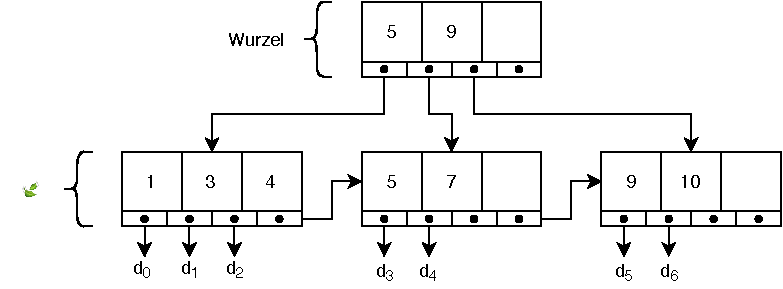
\includegraphics[scale=.5]{bplus_overview.pdf}
	

	
\end{columns}
\end{frame}
%------------------------------------------------



\begin{frame}
	\frametitle{Aufgabe 2.2 - Buffer Tree}
	\begin{columns}[c] % The "c" option specifies centered vertical alignment while the "t" option is used for top vertical alignment
		
		\column{.35\textwidth} % Left column and width
		\textbf{Operationen}
		\begin{enumerate}
			\item \textbf{search(7)}
			\item insert(x)
			\item delete(x)
		\end{enumerate}
		
		\column{.5\textwidth} % Right column and width
		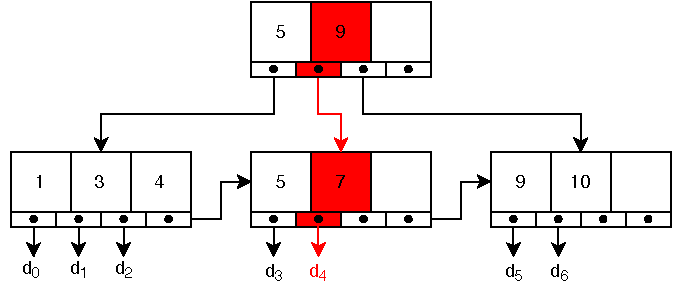
\includegraphics[scale=.6]{bplus_querry_7.pdf}
		
	
		
	\end{columns}
	\end{frame}
	%------------------------------------------------
	

	\begin{frame}
		\frametitle{Aufgabe 2.2 - Buffer Tree}
		\begin{columns}[c] % The "c" option specifies centered vertical alignment while the "t" option is used for top vertical alignment
			
			\column{.2\textwidth} % Left column and width
			\textbf{Operationen}
			\begin{enumerate}
				\item search(x)
				\item \textbf{insert(2)}
				\item delete(x)
			\end{enumerate}
			
			\column{.65\textwidth} % Right column and width
			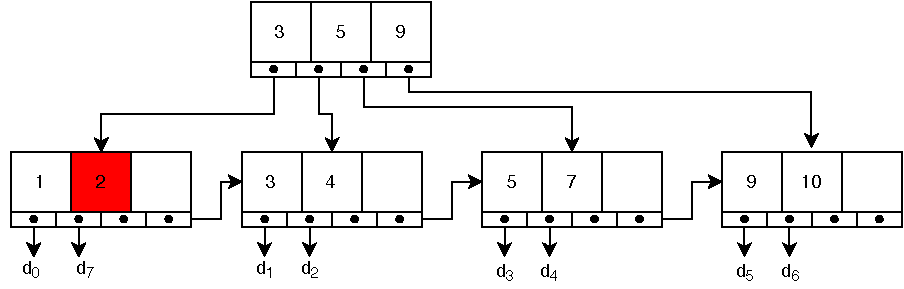
\includegraphics[scale=.6]{bplus_insert_2.pdf}
			
		
			
		\end{columns}
		\end{frame}
		%------------------------------------------------
		


\begin{frame}
\frametitle{Aufgabe 2.2 - Buffer Tree}
\begin{columns}[c] % The "c" option specifies centered vertical alignment while the "t" option is used for top vertical alignment
	
	\column{.2\textwidth} % Left column and width
	\textbf{Operationen}
	\begin{enumerate}
		\item search(x)
		\item insert(x)
		\item \textbf{delete(9)}
	\end{enumerate}
	
	\column{.65\textwidth} % Right column and width
	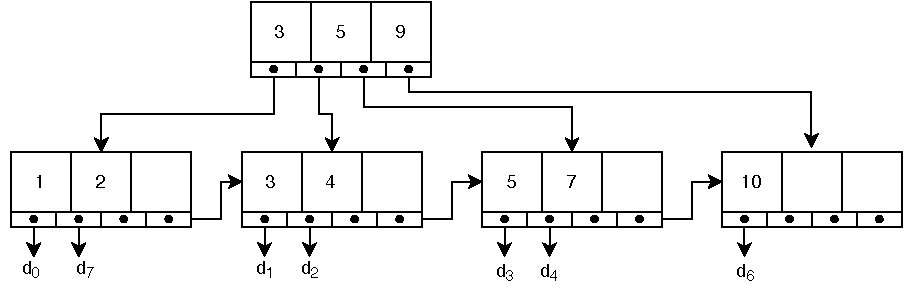
\includegraphics[scale=.6]{bplus_delete_9.pdf}
	

	
\end{columns}
\end{frame}
%------------------------------------------------
	



\begin{frame}
\frametitle{Aufgabe 2.2 - Buffer Tree}
\begin{columns}[c] % The "c" option specifies centered vertical alignment while the "t" option is used for top vertical alignment
	
	\column{.2\textwidth} % Left column and width
	\textbf{Operationen}
	\begin{enumerate}
		\item search(x)
		\item insert(x)
		\item \textbf{delete(9)}
	\end{enumerate}
	
	\column{.65\textwidth} % Right column and width
	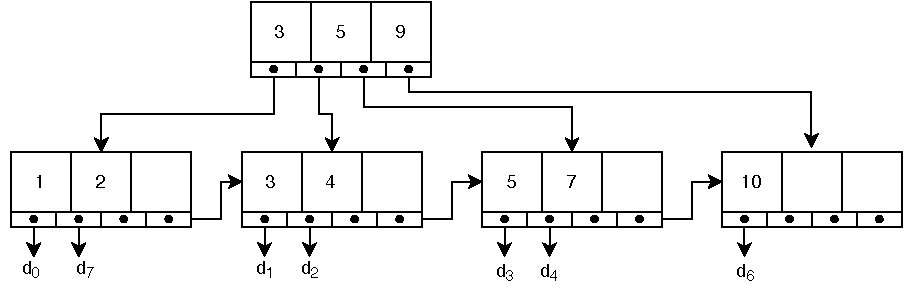
\includegraphics[scale=.6]{bplus_delete_9.pdf}
	

	
\end{columns}
\end{frame}
%------------------------------------------------



\begin{frame}
\frametitle{Aufgabe 2.2 - Buffer Tree}
\begin{columns}[c] % The "c" option specifies centered vertical alignment while the "t" option is used for top vertical alignment
	
	\column{.45\textwidth} % Left column and width
	\textbf{Buffer Tree}
	\begin{itemize}
		\item (a,b)-Baum mit $a=m/4$ und $b=m$
		\item $m:=$ größe des Buffers
		\item Tiefe $\mathcal{O}(\log_{m}(n))$
		\item $n$ Blätter je $\Theta(B)$
		\item Speicher $\mathcal{O}(n)$
		\item jeder Knoten bekommt Buffer
	\end{itemize}
	
	\column{.50\textwidth} % Right column and width
	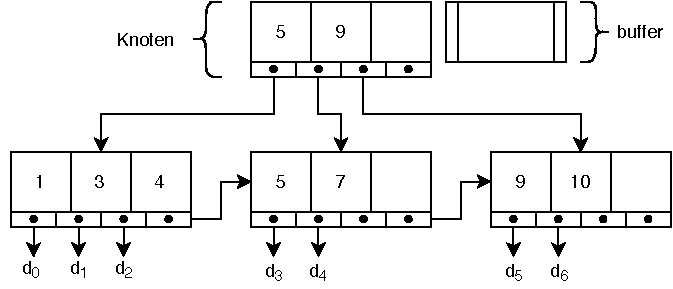
\includegraphics[scale=.55]{bufffer_tree_overview.pdf}
	

	
\end{columns}
\end{frame}
%------------------------------------------------
			

\begin{frame}
\frametitle{Aufgabe 2.2 - Buffer Tree}
\begin{columns}[c] % The "c" option specifies centered vertical alignment while the "t" option is used for top vertical alignment
	
	\column{.95\textwidth} % Left column and width
	\textbf{Buffer Tree}
	\begin{itemize}
		\item Operationen werden nicht sofort ausgeführt
		\item erzeugen Tupel [Element, Operation, Zeitstempel]
		\item wenn Anzahl Tupel $ \geq B \rightarrow$ Tupel in Buffer der Wurzel
		\item wenn Anzahl Tupel in Buffer $> m \rightarrow $ starte Buffer-Entleerungsprozess
	\end{itemize}
	

	
\end{columns}
\end{frame}
%------------------------------------------------
				

\begin{frame}
\frametitle{Aufgabe 2.2 - Buffer Tree}
\begin{columns}[c] % The "c" option specifies centered vertical alignment while the "t" option is used for top vertical alignment
	
	\column{.95\textwidth} % Left column and width
	\textbf{Buffer-Entleerungsprozess}
	\begin{itemize}
		\item interne Knoten $:=$ Knoten die keine Blätter als Kinder haben
		\item Blattknoten $:=$ Knoten deren Kinder Blätter sind
	\end{itemize}
	

	
\end{columns}
\end{frame}
%------------------------------------------------

			

\begin{frame}
\frametitle{Aufgabe 2.2 - Buffer Tree}
\begin{columns}[c] % The "c" option specifies centered vertical alignment while the "t" option is used for top vertical alignment
	
	\column{.95\textwidth} % Left column and width
	\textbf{Buffer-Entleerungsprozess: interne Knoten}
	\begin{itemize}
		\item Lade jeweils $M$ Tupel aus dem Buffer in den Hauptspeicher
		\item sortieren und mergen
		\item entferne Operationen die sich aufheben $\rightarrow$ insert(x), delete(x)
		\item verschiebe Tupel entsprechend ihrer Elemente in Buffer der Kinder
		\item starte Entleerungsprozess rekursiv für tiefere Buffer mit mehr als $m$ Elementen
	\end{itemize}
	

	
\end{columns}
\end{frame}
%------------------------------------------------

	

\begin{frame}
\frametitle{Aufgabe 2.2 - Buffer Tree}
\begin{columns}[c] % The "c" option specifies centered vertical alignment while the "t" option is used for top vertical alignment
	
	\column{.95\textwidth} % Left column and width
	\textbf{Buffer-Entleerungsprozess: Blattknoten}
	\begin{itemize}
	\item Lade Tupel aus Blattknoten mit zugehörigen Blättern in den Hauptspeicher
	\item Führe Operationen gemäß der Tupel aus
	\item schreibe Änderungen in den (a,b)-Baum zurück
	\end{itemize}
	

	
\end{columns}
\end{frame}
%------------------------------------------------
							
												
\begin{frame}
\frametitle{Aufgabe 2.2 - Buffer Tree}
\begin{columns}[c] % The "c" option specifies centered vertical alignment while the "t" option is used for top vertical alignment
	
	\column{.95\textwidth} % Left column and width
	\textbf{I/O Analyse}
	\begin{itemize}
	\item Sequenz von $N$ Operationen $\rightarrow \mathcal{O}(n\cdot \log_{m} n)$ I/Os
	\item Kosten Operation $\rightarrow\mathcal{O}((\log_{m} n)/B)$ I/Os amortisiert
	\item Buffer Tree benötigt $\mathcal{O}(n)$ Speicher
	\item ein Buffer Tree kann I/O optimal sortieren $\rightarrow\mathcal{O}(n\cdot \log_{m} n)$ I/Os
	\end{itemize}
	

	
\end{columns}
\end{frame}
%------------------------------------------------
									
							

\end{document} 